\documentclass[11pt]{article}
\usepackage{geometry}                
\geometry{letterpaper}                   

\usepackage{listings}
\usepackage{color}
\usepackage{graphicx}
\usepackage{epstopdf}
\usepackage{varioref}
\usepackage[numbers]{natbib}
\usepackage[squaren]{SIunits}
\usepackage{amssymb, amsmath}

\DeclareGraphicsRule{.tif}{png}{.png}{`convert #1 `dirname #1`/`basename #1 .tif`.png}

\title{Modelling Situations of Evacuation in a Multi-level Building}
\author{Hans Hardmeier, Andrin Jenal, Beat K\"ung & Felix Thaler}
\date{date} 

\begin{document}



\thispagestyle{empty}

\begin{center}

\includegraphics[width=5cm]{ETHlogo.eps}

\bigskip


\bigskip


\bigskip


\LARGE{ 	Lecture with Computer Exercises:\\ }
\LARGE{ Modelling and Simulating Social Systems with MATLAB\\}

\bigskip

\bigskip

\small{Project Report}\\

\bigskip

\bigskip

\bigskip

\bigskip


\begin{tabular}{|c|}
\hline
\\
\textbf{\LARGE{Insert Title Here}}\\
\textbf{\LARGE{...}}\\
\\
\hline
\end{tabular}
\bigskip

\bigskip

\bigskip

\LARGE{Name 1 \& Name 2}



\bigskip

\bigskip

\bigskip

\bigskip

\bigskip

\bigskip

\bigskip

\bigskip

Zurich\\
March 2012\\

\end{center}



\newpage

%%%%%%%%%%%%%%%%%%%%%%%%%%%%%%%%%%%%%%%%%%%%%%%%%

\newpage
\section*{Agreement for free-download}
\bigskip


\bigskip


\large We hereby agree to make our source code for this project freely available for download from the web pages of the SOMS chair. Furthermore, we assure that all source code is written by ourselves and is not violating any copyright restrictions.

\begin{center}

\bigskip
\bigskip
\bigskip
\bigskip


\begin{tabular}{@{}p{3.3cm}@{}p{6cm}@{}@{}p{6cm}@{}}

\begin{minipage}{3cm}

\end{minipage}
&
\begin{minipage}{6cm}
\vspace{2mm} \large Hans Hardmeier

 \vspace{\baselineskip}

\end{minipage}
&
\begin{minipage}{6cm}

\large Andrin Jenal

\end{minipage}

\end{tabular}

\bigskip
\bigskip
\bigskip
\bigskip


\begin{tabular}{@{}p{3.3cm}@{}p{6cm}@{}@{}p{6cm}@{}}

\begin{minipage}{3cm}

\end{minipage}
&
\begin{minipage}{6cm}
\vspace{2mm} \large Beat K\"ung

 \vspace{\baselineskip}

\end{minipage}
&
\begin{minipage}{6cm}

\large Felix Thaler

\end{minipage}
\end{tabular}

\end{center}
\newpage

%%%%%%%%%%%%%%%%%%%%%%%%%%%%%%%%%%%%%%%



% IMPORTANT
% you MUST include the ETH declaration of originality here; it is available for download on the course website or at http://www.ethz.ch/faculty/exams/plagiarism/index_EN; it can be printed as pdf and should be filled out in handwriting

%TODO: The is declaration of originality on the WEb for Windows (Andrin Jenal)...

%%%%%%%%%% Table of content %%%%%%%%%%%%%%%%%

\tableofcontents

\newpage

%%%%%%%%%%%%%%%%%%%%%%%%%%%%%%%%%%%%%%%



\section{Abstract}

If you are an ETH-Student, you know that at lunch time it is almost impossible 
to go out of the building through the main entrance to the polyterasse, because
of the number of students trying to leave at the same time. What would happen,
if in addition to that, a panic factor was involved? Have you ever imagined, how
an evacuation at the ETH Main building, ETH CAB-Building or even at your own home
would look like? How many people would be able to leave simultaneously? What is the
best strategy for people to leave? How would the perfect evacuation plan for your
school or enterprise building look like?

% [comment (Felix): we mention a panic factor but don't even simulate one? is this a good idea? :P]

In this work, we decided to elaborate a program that is flexible enough to
calculate the fastest exit for every given building structure. Using the "Fast
Sweeping Algorithm Method", introduced by James A. Sethian\cite{Zhao04afast} to
solve this complex problem, the program is capable of computing the fastest way
very efficiently.

% [comment (Felix): does not seem to be true. fast sweeping does not really help much.
% it is just used 2 times for initialization, the really time consuming simulation part is
% not influenced at all...

Different from all other similar projects, we also focused on an efficient and
realistic implementation of the program. Using our own data structures to
handle the numerous amount of agents and implementing the "Fast Sweeping
Algorithm Method" enables us to simulate large buildings with many agents and
with a realistic force model.

% [comment (Felix): Same here as above! nearly everything in the simulation code itself
% has a bigger influence on simulation time than fast sweeping! it's clearly nice to be able
% to use a 10000x10000 pixel image and have only some seconds of initialization time instead
% of some minutes with fast marching, but it does neither influence the total order of comlexity
% with respect to the number of agents (which is the limiting factor), nor does it save any times
% during the simulation phase, as it is not used there.]


\section{Individual contributions}

We all worked together in this project and used the individual strengths of each
of us to achieve the best possible result. Detailed information about the
contribution of each of us can be obtained from the git history.

%@hans: du chonsch an erschter stell
On the other hand Carl Hans Peter Hardmeier Samame, alias Hans Hardmeier, was 
responsible for some parts of the documentation, verification of the MATLAB-code
and calculating efficienty using different operating systems (i.e. Mac OS 10.6).

%todo: andrin
I did some drawings.


Beat K\"ung did most of the plotting functionality and the definition \&
implementation of the configuration and building image file. He also did several
sections of the documentation.

Felix Thaler implemented the algorithms written in \textit{C}, using \textit{MATLAB}'s \textit{MEX}-interface.
These are efficient \textit{Fast Sweeping}, a 2D \textit{Range Tree} and fast bilinear interpolation.
Further he developed the basic simulation framework and added the social force model as well as some
custom algorithms, for instance one to minimize wall penetration of agents. Some sections of the documentation are
written by him, too.


\section{Introduction and Motivations}

\subsection{Introduction}

Simulating the evacuation scenario of a single-level building is well known but
is not general enough. Though we want to introduce a more sophisticated
simulation within a multi-level building. E.g.: What would happen, if a
multi-level building has to be evacuated? Which escape routes would be mostly
used? Which effects would have the pressure/panic of other persons to the
situation? Since tower buildings are getting more common in large cities,
engineers have to care more about the behaviour in situations of emergency,
namely evacuations. Apart of the mathematical model and implementation for
solving this problem, we also wanted to increase the utility of this program for
all readers by giving the possibility of calculate different scenarios in
different buildings given by the user. In this work, we will mostly work with
the map of the ETH building, however, there are more configurations in the data
folder and one can replace any map with others that meet the properties of the
Figure \ref{building floor image} in the section \ref{matlab code}.

\subsection{Motivation}

Intuitive expectations and mathematical model results can stay sometimes in
contradiction. As ETH-Students the safety of the people inside the ETH building
is very important. But on the one hand, we are not sure, if the evacuation
potential of the building is enough for the amount of students during a normal
week day and on the other hand, we want to help the people around the world,
that have a similar question, to find an answer. This two points gave us the
ideas and motivation to create a flexible tool that simulates a real-world
scenario for any given building or even structures (i.e. planes or boats).

% [comment (Felix): special sentence: 'As ETH-Students...'. what the hell is a 'evacuation potential'
% 'we want to help the people around the world'??? really? i don't. i just wanted to get my credit points and some fun with coding.] 

\subsection{Fundamental Questions}

In the first place, we want to learn about how the humans behave under pressure
through already existing papers \cite{AACIBF} \cite{ACPPD}  \cite{SDFEP}
\cite{DCD} and find \textit{ what are the most influential forces, which decide
this kind of behavior.} Important is also the evaluation of the evacuation
potential of the given building and \textit{find places in the building that do
contribute on a crucial part to a panic behaviour}.  After the evaluation, we
want to \textit{compare our results with the corresponding results in the
literature} and find every single coherence and explain differences. Beside the
socio-phychological aspects of this problem, we also want to take a closer look
to the technical part and \textit{find the similarities to a single level
evacuation bottleneck problem}.

% [comment (Felix): we did not do most of the parts described here!!!]

\section{Description of the Model}
\subsection{General Model}

For our model, we will create a relatively general framework for behavioral
simulation in evacuation scenarios based on the social force model introduced by Dirk Helbling \cite{SDFEP}.
A core investigation is a simulation, beginning in a general everyday situation,
where people are spread randomly in their office or somewhere in the hallway and ending in an evacuation scenario.
At the end we should be able to make strong
statements anwsering our fundamental questions.
Based on the forces explained in the following paragraphs, we tried to figure
out how agents overcome major obstacles like tiny passages, stairs or pillars. Hence, the
shape and complexity of rooms and building is a key factor, contributing to the behaviour of the
agents as well. 

% [comment (Felix): 'strong statements anwsering our fundamental questions'? we don't even tried to answer the 'fundamental questions' described above!!] 

\subsection {Forces}
The reactions of the agents will mainly be influenced by different forces, model
parameters and the building structure itself. 
Describing this problem in mathematical terms, leads to an equation, where the mass, the desired direction $F_{D}$, the repulsive forces $F_{R}$ and the wall force $F_{W}$ of each individual agent contribute to the change of velocity in time.

\begin{equation} \label{eq:eikonal}
m\frac{\mathsf{d}\mathbf{v}}{\mathsf{d}t}=mF_{D}+\sum{F_{R}}+\sum{F_{W}}
\end{equation}

That means the change of position $\mathbf{r}$ is given by the velocity: $\mathbf{v}=\frac{\mathsf{d}\mathbf{r}}{\mathsf{d}t}$\\
To understand the different party, they will be explained briefly.

% [comment (Felix): we need to write MUCH more cleary that all these forces are exactly the same as the one proposed by Helbling!! This is my no means our work!]

\subsubsection{Desired Direction}

% [comment (Felix): ääääh somewhat short?? :-P]
\begin{equation} \label{eq:eikonal}
F_{D}=m\frac{v(t)\mathbf{e(t)}-\mathbf{v(t)}}{\tau}
\end{equation}

\subsubsection{Repulsive Interaction Force}
As poeple don't like to get too close to each other, the main component of this formula is a rather psychological aspect and plays an important role to keep agents apart from each other. Altohough if it should happen that agents get too close, two additional forces, the 'body force' counteracting body compression and 'sliding friction force' contribute to the repulsive force to ensure a certain distance. (ACHTUNG ZITIERT!) \\
ODER SO?! \\ % [comment (Felix): as mentioned above: no plagiarism and better orthography, PLEASE!]
Within an evacuation scenario, the psychological tendency of two pedestrians i
and j to stay away from each other, depends on the level of repulsion between
this two specific agents (margin of unconscious privacy area conservation
between them). In addition, we assume two other more physical forces: a `body
force' that counteracts the body compression between the agents (important
factor in a panic evacuation model) and a `sliding friction force' avoiding the
unnatural regulation of the speed when the agent nears another. \cite{SFMPD}

Quote from 'Helbling, Dirk - Molnar, Peter (1995): Social Force Model for Pedestrians Dynamics' \cite{SFMPD} :
\begin{center}
\textit{"The desired velocity $v^0_i$ can reach more than $5 \meter\second^{-1}$
(up to $10 \meter\second^{-1}$), but the observed free velocities for leaving a 
room correspond to $v^0_i=6 \meter\second^{-1}$ under relaxed, $1\meter\second^{-1}$
under normal, and $1.5\meter\second^{-1}$ under nervous conditions. A reasonable
estimate for the acceleration time is $0.5\meter\second^{-1}$."}
\end{center}
In our model, although the mass is not visible, it is important for
the calculation of the force of each agent. It's well known that the inertia of
each agent is directly dependent from his mass and velocity..

% [comment (Felix): what does 'not visible' mean? you can clearly see the difference between a simulation
% with higher or lower mass as long as all the other parameters stay the same...]

\subsubsection{Wall Force}

Using the nearest point on a wall to an agent, the repulsive forces created by
the whole wall is treaten analog as the created Agents-Repulsion-Forces (using a
fix force for each point in every wall, assuming that a wooden wall creates the
same repulsion as a paper wall or concrete wall). In the preprocesing, the walls
also represent points in the graph that cannot be reached, creating a 'natural'
gradient field all over the map showing the direction to the nearest exit. If in
the current floor there exists no exit, then stairs down are interpretend as the
local exits, hence the highest local point of attraction. \cite{SFMPD} 
-> formula

%%Evtl.  example of field force?? from /images Beat? Andrin? Felix?
% [comment (Felix): wall force don't have anything to do with the exits, the forces are calculated separately.
% the fast sweeping algorithm is used here with different boundary conditions, independent of anything other than the walls...
% what graph is meant? there's not really a 'graph' used anywhere...  what's a 'natural' gradient field???]


\section{Implementation}
Our goal was a fast implementation of the model. So we decided to use the Fast
Sweeping algorithm instead of the Fast Marching alorithm to calculate the
fastest way out of a building. We knew that \textit{MATLAB} code is not very fast and
\textit{MATLAB} provides an interface for other programming languages. So we
used the \textit{C} programming language to implement the Fast Sweeping method.

Later in the development process we discovered another bottleneck in our code:
The social force between the agents which runs in $ O(N^2) $. Felix Thaler then
introduced a Range Tree for this problem, which he also implemented in
\textit{C}.

% [comment (Felix): I would not mention fast sweeping here, as it's not really important for
% the overall performance and just described below...]

\subsection{\textit{MATLAB} Code} \label{matlab code}
We wanted to create a flexibel model which can be used to simulate every
possible building structure.

% [comment (Felix): it's not possible at all to simulate 'every possible' building.
% what about some reformulation? ]

Each scenario is described in a configuration file. This includes for example how many
agents are placed on each floor or the timestep of the simulation (the exact
definition can be found in the file data/config\_file\_structure). Each config
file also references one or more building floor images.
Figure \vref{building floor image} describes how a building floor
image must look like. The agents are placed randomly within the agents spawning
area(s).

\begin{figure}[h]
\centering
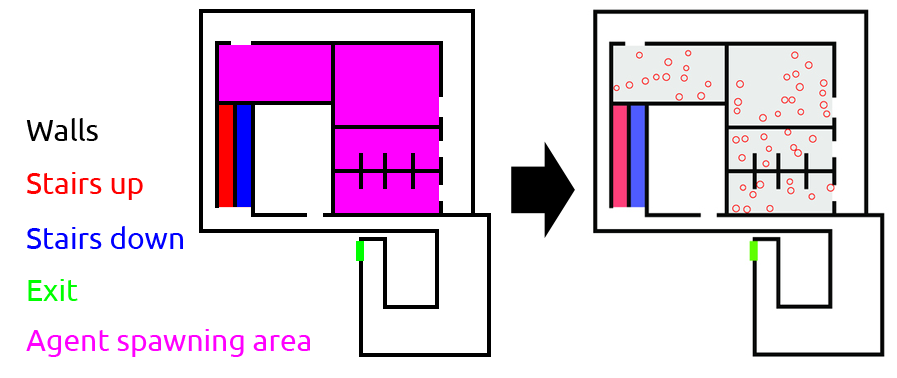
\includegraphics[width=\textwidth]{./images/config_floor_description.png}
\caption{Left the building floor image and right how it looks when the
simulation is running} 
\label{building floor image}
\end{figure}

Since \textit{MATLAB} is not really object-oriented, we used a big data structure (called
data) that includes all internal data that we use (eg. the floors and agents).
It is passed as an argument for every function that needs it.

\subsection{Pathfinding}
As described in \cite{SFMPD}, the agents always try to reach their desired destination
using the shortest possible path. As we use raster graphics to encode simulation data,
we decided to use the same discrete grid to compute the nearest path to an exit for every point approximately.
Mathematically, this can be expressed as an partial differential equation, the 2D Eikonal equation (equation \ref{eq:eikonal}).

\begin{equation} \label{eq:eikonal}
\|\mathbf{\nabla} d(\mathbf{x})\|=1 \quad d:\!\mathbb{R}^{2}\to\mathbb{R},\mathbf{x}\in\mathbb{R}^{2}
\end{equation}

The solution $d(\mathbf{x})$ now gives the distance to the nearest exit point, its
negative gradient $-\mathbf{\nabla}d(\mathbf{x})$ therefor always points in the 
direction of the shortest path towards the desired exit. There are mainly two
competitive agorithms for solving this equation efficiently. First there is the
\textit{Fast Marching} method, a specialized version of Dijkstra's well known 
algorithm \cite{dijkstra59a}. The alternative is \textit{Fast Sweeping}, which 
leads to a much simpler implementation, faster calculation and better algorithmic
complexity of $O(n)$ instead of $O(n\log n)$ with respect to the discretization size.
We therefor implemented an efficient \textit{Fast Sweeping} method, closly following
\cite{Zhao04afast} as a basis of our pathfinding and repulsive wall forces. The 
algorithm uses an upwind finite difference scheme where our mesh is defined by 
the input images. The implementation was done \textit{C} and not directly in
\textit{MATLAB}, using optimized boundary condition handling for our pruposes.
Our benchmarks showed a high speed increase compared to other Eikonal solvers,
e.g. the "Accurate Fast Marching" implementation as found at \textit{MATLAB CENTRAL}
\cite{fastmarching}.

% [comment (Felix): do we want to merge this subsection with the one about the 'desired force'?]


\subsection{Profiling \& Optimization}

%TODO: 
% profiler resultat diskutieren
%  addAgentRepulsiveForce langsam, da N^2
% [comment (Felix): not anymore N^2, but N*log(N)^2, some info is already in section 'implementation' as well as in the subsection 'range tree']


Using the \textit{Profiler}-function of \textit{MATLAB}, we were able to discuss
the efficiency of our implementation. The following image show the time comsumption
for the calculation of the evacuation of 2 floors (ETH CAB-Building Floors E and F) within x seconds:
%Running write seconds...

\begin{figure}[h]
\centering
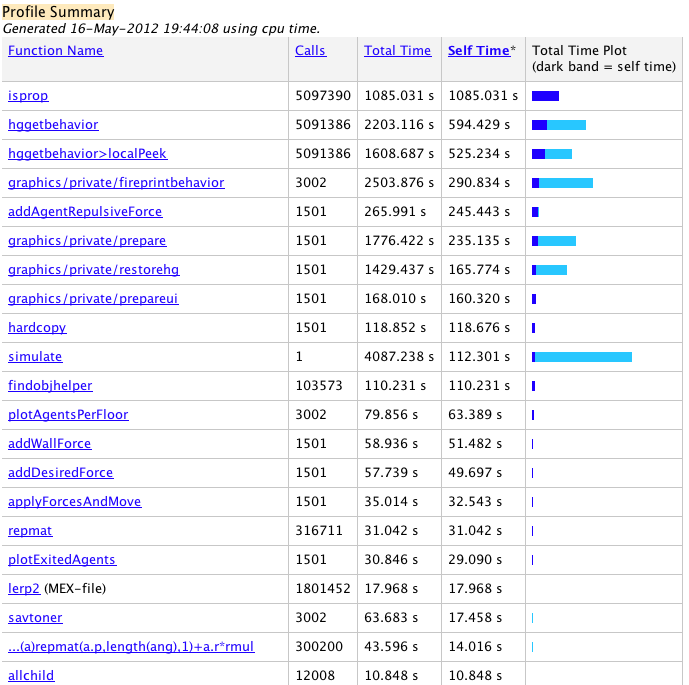
\includegraphics[width=0.8\textwidth]{./images/profiler.png}
\caption{Profile of the calculation for the CAB-Building with 300 agents over 3 different floors} 
\label{cab profile}
\end{figure}


\subsubsection{Parallelization}

We tried to optimize the code using the parallel for-loop parfor in \textit{MATLAB}. In
the function applyForcesAndMove we replaced the for-loop over the agents with
parfor. We measured the time using an input with 200 agents on a 4 core machine
using 5 \textit{MATLAB} workers. The result was that the parfor version was even slightly
slower than the serial version. The reason for this is how \textit{MATLAB} implements
parfor: all the memory that is used by a worker must be sent to this worker.
Each agent must access the building floor image randomly and this creates a
large amount of memory that must be transferred to each worker, which leads to a
decreasing performance.
This is why we decided not to use parfor or any other parallelization in our
implementation.

% [comment (Felix): perhaps it's not really clear what parfor actually is...]

\subsubsection{Improving default commands}

Through our first messures, we realised that the function \verb+interp2+
consumed a lot of resources and time. We decided to create our own operator
called \verb+lerp2+ (written in \textit{C}) that interpolates between data points. It finds values of a
two-dimensional function underlying the data at intermediate points bilinearly.
Here the different given data points are the current values of the frame $i-1$
for the frame $i$. 
%TODO: More Details lerp2.
% [comment (Felix): really more details? who cares about bilinear interpolation? :)
% perhaps it's not fully clear that interp2 is a off-the-shelf MATLAB function?
% and what's about a different title? something with 'replacement' isntead of
% 'improvement' would probably be more accurate...]

\begin{figure}[h]
\centering
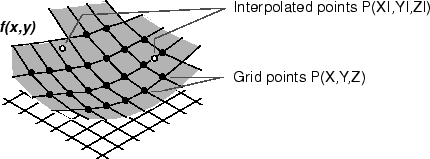
\includegraphics[width=0.5\textwidth]{./images/lerp2.png}
\caption{Visualisation of lerp2.c} 
\label{lerp2 image}
\end{figure}

% [comment (Felix): we need the SOURCE of this image!! or is it somewhere stated?]

\subsubsection{Range Tree}
The most time consuming part in our program is the calculation of the interaction
forces between the agents, at least if their count is high enough. To reduce the
natural complexity of order $O(n^{2})$ of this inter-agent interaction, we can clamp forces
with little effect, e.g. in our implementation all forces smaller than $ 10^{4}\newton$.
As their exponentially decreasing, the distance in which the forces need to be adressed
is only several meters, so a big part of them can just be ignored without introducing 
a significant error.

To get all agents influenced by another agent by a force bigger than a threshold, we need to be able
to search neighbours of any agent within a given distance. To efficiently query 
these agents, we implemented a 2D \textit{Range Tree} in \textit{C}, which allows query times
of order $O(\log^{2} n+k)$, where $n$ is the total number of agents and $k$ is the number of
queried agents \cite{algdat}. In larger simulations this reduces simulation times by a significant factor.

\section{Simulation Results and Discussion}

\subsection{Expected Results}

We expect the stairs and the main building exit to be the bottlenecks. The
amount of people in lower levels is increasing with time until a certain point,
when most of the people have exited the building. Also we think that if the 
velocity of the people is higher (people are more in panic), jams at the
exit will increase and people will mainly try to take the main exit instead of
emergency exits.

% [comment (Felix): don't know if that's relevant, but our agents always try to choose
% the nearest exit, no matter how many agents already try to escpape there...]

\subsection{Simulation Results}

As expected the main exit becomes a bottleneck...
%TODO: Discussion

\begin{figure}[h]
\centering
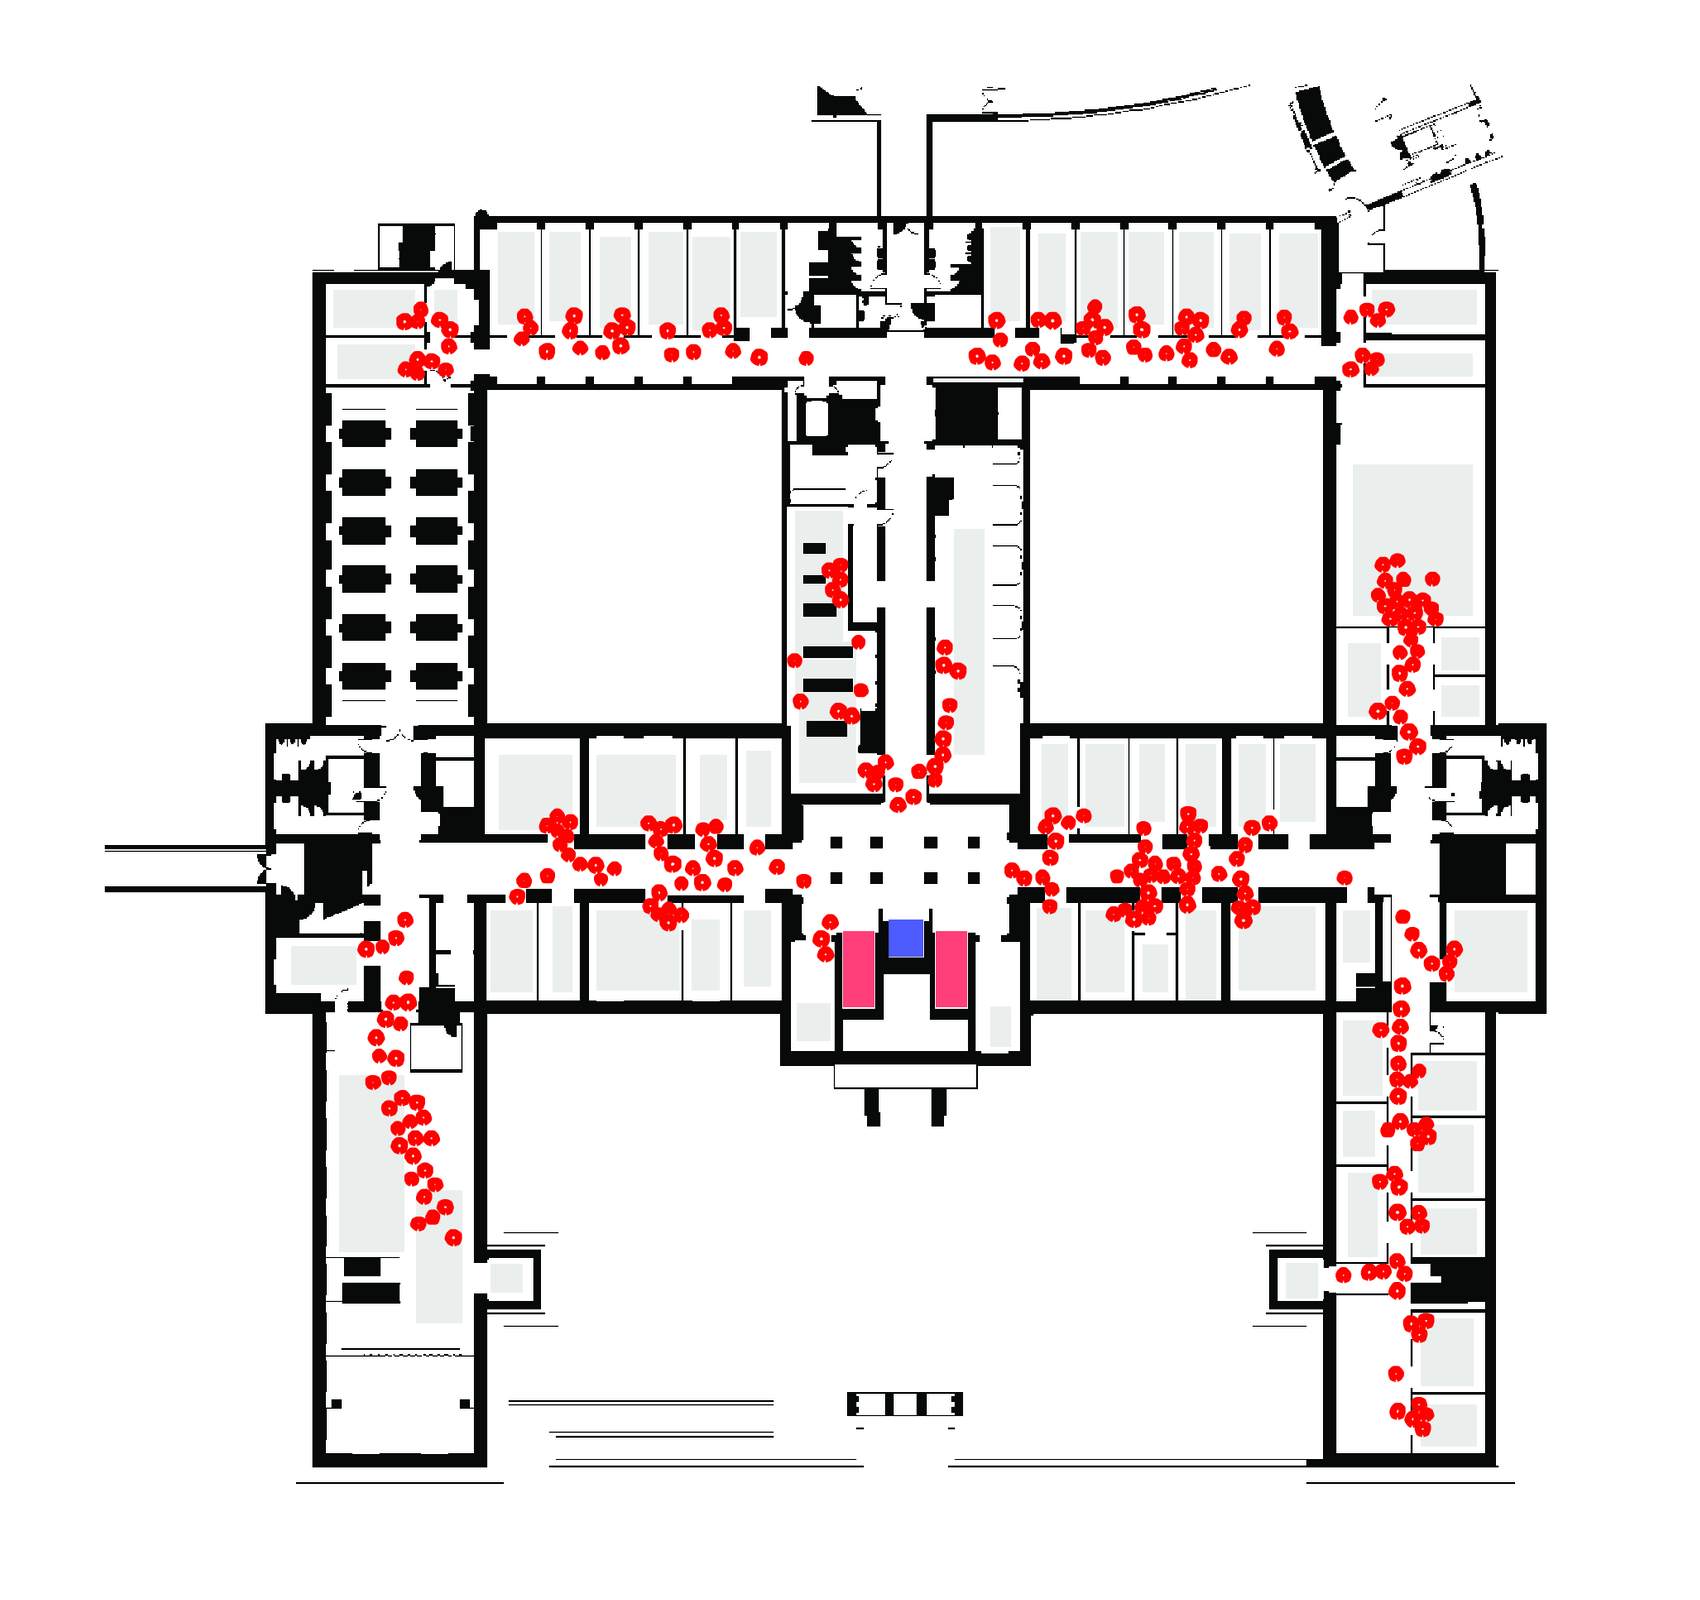
\includegraphics[width=0.8\textwidth]{./images/cab1.png}
\caption{Visualisation of evacuation in the CAB Building E Floor} 
\label{cab1}
\end{figure}



%TODO: add some plots, ...

\subsection{Discussion}


\section{Summary and Outlook}

In this section we would like to thank the MSSSM-Group from the ETH in Zurich, Switzerland
directed by Karsten Donnay and Stefano Balietti for their engagement in the lecture
"Modeling and Simulating Social Systems with \textit{MATLAB}" during the Spring Semester 2012.
This project helped us to understand that the human behavior is a difficult subject to formalize.
Non expected reactions (i.e. paranoia, desesperation or creativity) have not been consider by
making this model and we are sure that in the reality this factors have also a big importance.
This is a point where this work could be improved. Nevertheless, we believe that this project
gives a good prespective in matters of evacuation potential and security.


%TODO: Rückblick aufs projekt & Danksagung

\section{References}

\begin{thebibliography} {9}
	
	\bibitem{Zhao04afast} Zhao, Hongkai (2004): A Fast Sweeping Method for Eikonal Equations.
	\bibitem{SFMPD} Helbling, Dirk - Molnar, Peter (1995): Social Force Model for Pedestrians Dynamics.
	\bibitem{AACIBF} Helbling, Dirk, Johansson, Anders (2006): Analytical Approach to Continuous and Intermittent Bottleneck Flows.
	\bibitem{ACPPD} Schadschneider, Andreas et al. (2002): CA Approach to Collective Phenomena in Pedestrian Dynamics.	
	\bibitem{DCD} Helbling, Dirk, Johansson, Anders (2007): Dynamics of crowd disasters: An empirical Study.
	\bibitem{SDFEP} Helbling, Dirk et al. (2000): Simulating dynamical features of escape panic.
	\bibitem{SPCD} Helbling, Dirk et al. (2005): Self-Organized Pedestrian Crowd Dynamics: Experiments, Simulations, and Design Solutions.
	\bibitem{dijkstra59a} Dijkstra, Edsger W. (1959): A Note on Two Problems in Connexion with Graphs.
	\bibitem{fastmarching} Kroon, Dirk-Jan (2011): http://www.mathworks.com/matlabcentral/fileexchange/24531-accurate-fast-marching
	\bibitem{algdat} Ottmann, Thomas, Widmayer, Peter (2002): Algorithmen und Datenstrukturen, 4. Auflage.

\end{thebibliography}

% use \cite{SFMPD} for citation

\section{Appendix}

\subsection{Code}

% define colors
\definecolor{commentcolor}{RGB}{89, 168, 89}
\definecolor{keywordcolor}{RGB}{68, 68, 255}
\definecolor{stringcolor}{RGB}{205, 139, 247}
\definecolor{numbercolor}{RGB}{128, 128, 128}
\definecolor{bgcolor}{RGB}{245, 248, 253}

% define listings style
\lstset{
  language=Matlab,
  basicstyle=\footnotesize\ttfamily,
  numbers=left,
  numberstyle=\tiny\color{numbercolor},
  stepnumber=2,
  numbersep=5pt,
  backgroundcolor=\color{bgcolor},
  showspaces=false, 
  showstringspaces=false,
  showtabs=false,
  frame=lines,
  rulecolor=\color{black},
  tabsize=2,
  captionpos=b,
  breaklines=true,
  breakatwhitespace=true,
  title=\lstname,
  commentstyle=\color{commentcolor},
  keywordstyle=\color{keywordcolor},
  stringstyle=\color{stringcolor}
}

\subsubsection{\textit{MATLAB} code}

% code is ordered alphabetically by file name...

\lstinputlisting[caption=addAgentRepulsiveForce.m]{../code/addAgentRepulsiveForce.m}
\lstinputlisting[caption=addDesiredForce.m]{../code/addDesiredForce.m}
\lstinputlisting[caption=addWallForce.m]{../code/addWallForce.m}
\lstinputlisting[caption=applyForcesAndMove.m]{../code/applyForcesAndMove.m}
\lstinputlisting[caption=checkForIntersection.m]{../code/checkForIntersection.m}
\lstinputlisting[caption=compileC.m]{../code/compileC.m}
\lstinputlisting[caption=initAgents.m]{../code/initAgents.m}
\lstinputlisting[caption=initEscapeRoutes.m]{../code/initEscapeRoutes.m}
\lstinputlisting[caption=initialize.m]{../code/initialize.m}
\lstinputlisting[caption=initWallForces.m]{../code/initWallForces.m}
\lstinputlisting[caption=loadConfig.m]{../code/loadConfig.m}
\lstinputlisting[caption=plotAgentsPerFloor.m]{../code/plotAgentsPerFloor.m}
\lstinputlisting[caption=plotExitedAgents.m]{../code/plotExitedAgents.m}
\lstinputlisting[caption=plotFloor.m]{../code/plotFloor.m}
\lstinputlisting[caption=simulate.m]{../code/simulate.m}

\subsubsection{\textit{C} code}

\lstinputlisting[language=C,caption=createRangeTree.c]{../code/createRangeTree.c}
\lstinputlisting[language=C,caption=fastSweeping.c]{../code/fastSweeping.c}
\lstinputlisting[language=C,caption=getNormalizedGradient.c]{../code/getNormalizedGradient.c}
\lstinputlisting[language=C,caption=lerp2.c]{../code/lerp2.c}
\lstinputlisting[language=C,caption=rangeQuery.c]{../code/rangeQuery.c}
\lstinputlisting[language=C,caption=tree.h]{../code/tree.h}
\lstinputlisting[language=C,caption=tree\_build.h]{../code/tree_build.h}
\lstinputlisting[language=C,caption=tree\_build.c]{../code/tree_build.c}
\lstinputlisting[language=C,caption=tree\_free.c]{../code/tree_free.c}
\lstinputlisting[language=C,caption=tree\_query.h]{../code/tree_query.h}
\lstinputlisting[language=C,caption=tree\_query.c]{../code/tree_query.c}
\lstinputlisting[language=C,caption=tree\_types.h]{../code/tree_types.h}



\end{document}  



 
